% This LaTeX document needs to be compiled with XeLaTeX.
\documentclass[
  10
]{article}
\usepackage[margin=2cm,includehead=true,includefoot=true,centering,]{geometry}
\usepackage{xcolor}
\usepackage{ucharclasses}
\usepackage{hyperref}
\usepackage{amsmath,amssymb}
\usepackage{amsfonts}
\usepackage[version=4]{mhchem}
\usepackage{stmaryrd}
\usepackage{bbold}
\usepackage{polyglossia}
\usepackage{fontspec}
\usepackage{ctex}
\usepackage[export]{adjustbox}
\usepackage{tabularx}
\usepackage{booktabs}

\usepackage{setspace}
\setstretch{1.2}

\makeatletter
\@ifundefined{KOMAClassName}{% if non-KOMA class
  \IfFileExists{parskip.sty}{%
    \usepackage{parskip}
  }{% else
    \setlength{\parindent}{0pt}
    \setlength{\parskip}{6pt plus 2pt minus 1pt}}
}{% if KOMA class
  \KOMAoptions{parskip=half}}
\makeatother
\usepackage{longtable,booktabs,array}
\newcounter{none} % for unnumbered tables
\usepackage{calc} % for calculating minipage widths
% Correct order of tables after \paragraph or \subparagraph
\usepackage{etoolbox}
\makeatletter
\patchcmd\longtable{\par}{\if@noskipsec\mbox{}\fi\par}{}{}
\makeatother
% Allow footnotes in longtable head/foot
\IfFileExists{footnotehyper.sty}{\usepackage{footnotehyper}}{\usepackage{footnote}}
\makesavenoteenv{longtable}
\usepackage{graphicx}
\makeatletter
\newsavebox\pandoc@box
\newcommand*\pandocbounded[1]{% scales image to fit in text height/width
  \sbox\pandoc@box{#1}%
  \Gscale@div\@tempa{\textheight}{\dimexpr\ht\pandoc@box+\dp\pandoc@box\relax}%
  \Gscale@div\@tempb{\linewidth}{\wd\pandoc@box}%
  \ifdim\@tempb\p@<\@tempa\p@\let\@tempa\@tempb\fi% select the smaller of both
  \ifdim\@tempa\p@<\p@\scalebox{\@tempa}{\usebox\pandoc@box}%
  \else\usebox{\pandoc@box}%
  \fi%
}
% Set default figure placement to htbp
\def\fps@figure{htbp}
\makeatother
\setlength{\emergencystretch}{3em} % prevent overfull lines
\providecommand{\tightlist}{%
  \setlength{\itemsep}{0pt}\setlength{\parskip}{0pt}}


\hypersetup{colorlinks=true, linkcolor=blue, filecolor=magenta, urlcolor=cyan,}
\urlstyle{same}

\usepackage{colortbl}
\definecolor{table-row-color}{HTML}{999999}
\definecolor{table-rule-color}{HTML}{999999}
%\arrayrulecolor{black!40}
\arrayrulecolor{table-rule-color}     % color of \toprule, \midrule, \bottomrule
\setlength{\aboverulesep}{0pt}
\setlength{\belowrulesep}{0pt}


\setotherlanguages{english}
\IfFontExistsTF{Source Han Serif CN}
{\newfontfamily\chinesefont{Source Han Serif CN}}
{\IfFontExistsTF{Noto Serif CJK SC}
  {\newfontfamily\chinesefont{Noto Serif CJK SC}}
  {\IfFontExistsTF{SimSun}
    {\newfontfamily\chinesefont{SimSun}}
    {\IfFontExistsTF{FangSong}
      {\newfontfamily\chinesefont{FangSong}}
      {\newfontfamily\chinesefont{Arial Unicode MS}}
}}}
\IfFontExistsTF{Times New Roman}
{\newfontfamily\englishfont{Times New Roman}}
{\IfFontExistsTF{Liberation Serif}
  {\newfontfamily\englishfont{Liberation Serif}}
  {\IfFontExistsTF{DejaVu Serif}
    {\newfontfamily\englishfont{DejaVu Serif}}
    {\newfontfamily\englishfont{Arial}}
}}


\author{}
\date{}

\begin{document}


2022年全国大学生物理实验竞赛

\section{参赛项目说明书}\label{ux53c2ux8d5bux9879ux76eeux8bf4ux660eux4e66}

基于 U型锥形无芯光纤的透明液体浓度传感器的研制

\subsection{项目概述}\label{ux9879ux76eeux6982ux8ff0}

浓度是表征介质溶液特性的重要参数之一，物质的许多物理和化学性质均易受浓度的影响，浓度过高或者过低都会对产品的质量产生影响。因此对溶液浓度的测量与控制在造纸、化工、制糖、食品、制药等行业有着广泛的应用。目前，在透明溶液浓度的检测与控制方面，通过测量液体折射率来测量液体浓度是最常用的方法之一。常用的折射率的测量方法大致归纳为三类，即：几何光学法（阿贝折射计）、波动光学法（CCD自动测量法）以及光纤传感法。相比于其他两种方法，光纤传感法具有设备体积小、重量轻、耐腐蚀、抗电磁干扰、成本低廉等优点。鉴于此，本实验基于光纤的倏逝波传感原理，采用单模光纤-无芯光纤-单模光纤（SNS）结构，将待测液体作为无芯光纤的包层，制作成测量透明液体浓度的光纤传感探头，进行了液体浓度传感系统的设计与制作。为了提高灵敏度，对无芯光纤进行拉锥，制作了锥形无芯光纤的传感探头；在此基础上，为了进一步提高传感灵敏度，对锥形无芯光纤进行弯曲处理，制作了U型锥形无芯光纤传感探头。实验结果表明：以盐水溶液为测试对象，未拉锥的
SNS 结构光纤传感探头的传感灵敏度为
41.43nW/\%；锥形无芯光纤传感探头的灵敏度为
58.04nW/\%；U型锥形无芯光纤传感探头的灵敏度可以提高至
115.14nW/\%。从实验结果可以看出：采用拉锥和U型化处理后的无芯光纤可以大大提高透明液体浓度传感器的测试灵敏度。最后采用
STM32
单片机结合硬件电路、软件控制实现了盐水和酒精液体浓度的实时显示。实验结果表明，基于U型锥形无芯光纤的透明液体浓度测量系统可以完成恶劣环境下液体浓度的检测，且光电信号转换方便，便于多点采样，并可实现实时在线检测，是测量液体浓度的一种有效方法。

\subsection{1. 实验原理}\label{ux5b9eux9a8cux539fux7406}

\subsection{1.1
基于光纤倏逝波的传感原理}\label{ux57faux4e8eux5149ux7ea4ux500fux901dux6ce2ux7684ux4f20ux611fux539fux7406}

SNS全光纤传感探头结构如图 1所示。

\pandocbounded{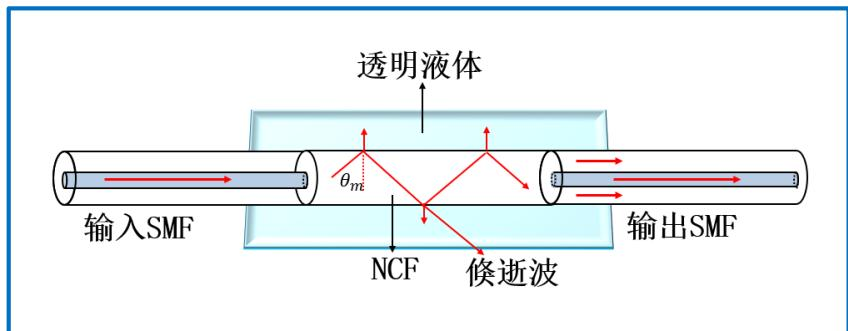
\includegraphics[keepaspectratio,alt={image}]{images/b7a263dc47ffca124b90f20e7e99624a7ad2ff42a9652e10e9a919e9fd65e761.jpg}}

图 1 SNS全光纤传感探头的结构

设�(�,0)为输入端单模光纤（SMF）中传输的基模光场，由于无芯光纤（NCF）的直径远大于SMF的纤芯直径，因此当输入光传输至NCF时，会在NCF中激发起多个模式
\(\{ \mathrm { L P _ { n m } } \}\) 。SMF 和 NCF
是无偏心对接，因为输入场及光纤结构具有中心对称性，因此只有
\(\left\{ \mathrm { L P _ { 0 m } } \right\}\) 模式被激发。在输入端
SMF和 NCF连接处，根据电磁场的连续性条件得到：

\[
E (r, 0) = \sum_ {m = 1} ^ {M} c _ {m} F _ {m} (r)\tag{1}
\]

式中�为NCF中激发模的总数， \(F _ { m } ( r )\)
是第�阶模式的光场，�为光纤横截面的径向坐标， \(c _ { m }\)
为第�阶模式的激发系数，其表达式为：

\[
c _ {m} = \frac {\int_ {0} ^ {\infty} E (r , 0) F _ {m} (r) r d r}{\int_ {0} ^ {\infty} F _ {m} (r) F _ {m} (r) r d r}\tag{2}
\]

因为 NCF 中传输的各阶模式在 NCF
与透明液体的界面上发生全反射，会在透入一定深度的透明液体中形成倏逝场，透明液体会对倏逝场有一定的衰减作用，所以当光波在NCF中传输�距离后，其光场可表示为：

\[
E (r, z) = \sum_ {m = 1} ^ {M} c _ {m} F _ {m} (r) \exp (i \beta_ {m} z) \exp (- \gamma_ {m} z)\tag{3}
\]

式中 \(\beta _ { m }\) 和 \(\gamma _ { m }\)
分别为第�阶模式的纵向传播常数和倏逝场吸收系数。

对于子午线入射情况， \(\gamma _ { m }\) 可表示为：

\[
\gamma_ {m} = \frac {\alpha_ {\lambda} \lambda n _ {f} c o s \theta_ {m} c o t \theta_ {m}}{4 \pi R _ {0} n _ {c} ^ {2} c o s ^ {2} \theta_ {c} \sqrt {s i n ^ {2} \theta_ {m} - s i n ^ {2} \theta_ {c}}}\tag{4}
\]

式中 \(\alpha _ { \lambda }\) 是 MF 在真空波长�处的消光系数，
\([ \theta _ { c } = a r c s i n ( n _ { f } / n _ { c } ) ]\) ，
\(\theta _ { c }\) 为传感区域的全反射临界角， \(n _ { f }\) 和
\(| n _ { c }\) 分别是透明液体和NCF的折射率， \(R _ { 0 }\)
是NCF的半径， \(\theta _ { m }\)
是传感区域中第m阶模式的光线相对于分界面法线的入射角，如图1所示。

光通过长度为�的 NCF 后再耦合到输出端 SMF
中，考虑到各个模式之间发生的干涉现象和透明液体对倏逝场的吸收作用，在波长�处的透射率可表示为：

\[
T (\lambda) = \sum_ {m \cdot n = 1} ^ {M} c _ {m} ^ {2} \cdot c _ {n} ^ {2} \cdot \cos [ (\beta_ {m} - \beta_ {n}) L ] \cdot \exp [ - (\gamma_ {m} + \gamma_ {n}) L ]\tag{5}
\]

由模式传播理论可知：透明液体折射率 \(n _ { f }\) 的变化会引起 NCF
中模式传播常数 \(\cdot \beta _ { m }\) 和激发系数 \(c _ { m }\)
的改变，由(4)式可知折射率 \(n _ { f }\) 和消光系数
\(\alpha _ { \lambda }\) 的变化均会引起倏逝场吸收系数
\(\cdot \gamma _ { m }\) 的变化。因为透明液体的折射率
\(\cdot n _ { f }\) 和消光系数 \(\alpha _ { \lambda }\)
均随浓度的变化而改变，所以(5)式中激发系数 \(c _ { m }\) 、模式干涉项
\(c o s \left[ ( \beta _ { m } - \beta _ { n } ) L \right]\) 和衰减项
\(e x p \left[ - ( \gamma _ { m } + \gamma _ { n } ) L \right]\)
均随着液体浓度的变化而变化，这样透射光谱也会随着液体浓度的变化而改变，具体反映在干涉项变化引起的特征峰的移动和三项共同作用引起的透射率变化。由模式传播理论和(4)式可知，影响透射谱透射率的激发系数
\(c _ { m }\) 、模式传播常数 \(\cdot \beta _ { m }\) 和倏逝场衰减系数
\(\cdot \gamma _ { m }\)
均与波长�有关，因此在其他参数相同的条件下，相同的液体浓度下不同波长处的传输损耗不同；同样在液体浓度相同的条件下，不同波长处透射损耗的变化也不同。因此，可以通过透射谱特征波长的移动和传感探头透射功率的变化来检测液体的浓度。

\subsection{1.2锥形
NCF传感增敏原理}\label{ux9525ux5f62-ncfux4f20ux611fux589eux654fux539fux7406}

锥形光纤示意图如图
2所示。某一特定波长的光从锥形光纤的大端面向小端面入射时，入射角
\(\alpha _ { n }\) 随次数�增加而不断减小，如图
2（a）所示，根据倏逝波的定义可知穿透深度为：

\[
d _ {t} = \frac {\lambda}{2 \pi \sqrt {n _ {1} ^ {2} s i n ^ {2} \theta_ {i} - n _ {2} ^ {2}}}\tag{6}
\]

由此可知，在波长一定情况下，随反射次数的增加 \(\mid d _ { t }\)
不断增大。在接近临界角的情况下，倏逝波的穿透深度急剧增大。某一特定波长的光从锥形光纤的小端面向大端面入射时，如图
（ ）所示，由公式（ ）可知，随着反射次数的增加之
\(\scriptstyle d _ { t }\) 不断减小。在接近 \(9 0 ^ { \circ }\)
°的情况下，倏逝波的穿透深度趋于平稳，对光的束缚能力也达到最大。倏逝波穿透深度决定了光场能量泄露与外界物质的相互作用的大小。因此，采用锥形光纤增加倏逝波的穿透深度，可以提高透明液体浓度传感器的灵敏度。

\pandocbounded{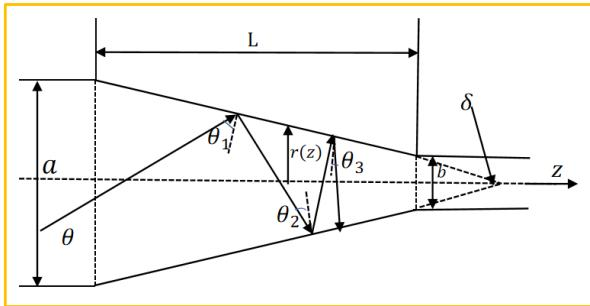
\includegraphics[keepaspectratio,alt={image}]{images/0ee99bad753ff4e2b5f06199edf6ac2da00ab9565de6cc5c58c4af6db4412e69.jpg}}

（a）

\pandocbounded{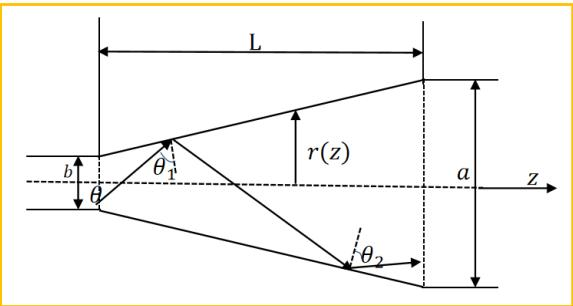
\includegraphics[keepaspectratio,alt={image}]{images/3ebce4438d8c948dc542f1c4e2974a3adb56ec182f7610cafd9263b6dcb66cf0.jpg}}

（b）

图 2 锥形光纤示意图

（a）光波从大端面向小端面入射

（b）光波从小端面向大端面入射

\subsection{1.3 U型锥形
NCF传感增敏原理}\label{uux578bux9525ux5f62-ncfux4f20ux611fux589eux654fux539fux7406}

当光场在弯曲光纤中传输时，纤芯中导模倏逝场边缘部分的传输常量与包层模相同时，基模的倏逝场耦合成包层模，包层模在传输过程不断损耗，形成弯曲损耗。弯曲光纤的弯曲半径越小，经过纤芯导模的倏逝场耦合到包层的光场越多，造成的损耗也就越大。但是，并非所有耦合到包层的光场都损耗掉了，其中部分包层模式又会耦合回纤芯，与纤芯中的导模发生干涉。因此，采用U型锥形光纤可以进一步提高透明液体浓度传感器的灵敏度。

\subsection{1.4
三种结构光场分布的模拟仿真}\label{ux4e09ux79cdux7ed3ux6784ux5149ux573aux5206ux5e03ux7684ux6a21ux62dfux4effux771f}

采用光束传播法(BPM)仿真基于 NCF、锥形 NCF以及 U型锥形
NCF的三种传感探头的光场分布，仿真参数如表 1所示。

表 1 仿真参数

{\def\LTcaptype{none} % do not increment counter
\begin{longtable}[]{@{}|l|l|@{}}
\toprule\noalign{}
\endhead
\bottomrule\noalign{}
\endlastfoot
\hline
波长(nm) & 1550 \\
\hline
背景折射率 & 1 \\
\hline
输入/输出 SMF 的长度 (μm) & 1000 \\
\hline
SMF 的纤芯/包层直径 (μm) & 8.2/125 \\
\hline
SMF 的纤芯/包层折射率 RI & 1.45205/1.44681 \\
\hline
NCF 的长度 (μm) & 44000 \\
\hline
NCF 的直径 (μm) & 125 \\
\hline
NCF 的折射率 RI & 1.444 \\
\hline
锥形 NCF 的最小直径 (μm) & 20 \\
\hline
U 型锥形 NCF 的弯曲角度 (°) & 大约 60 \\
\hline
\end{longtable}
}

三种结构的纵向和横向光场分布如图3所示。可以看出，NCF的传输原理是多模干涉，具有最大透射光能的两点之间的距离是自成像周期。为了获得更大的输出光强，

NCF的长度应该是自成像周期的整数倍。所以在该实验中NCF的长度取为4.4厘米。图3（a）和（b）是采用NCF的传感结构中纵向和横向的光场分布。可以看出，在NCF外有非常小的倏逝波场。采用锥形NCF的传感结构的光场分布如图3（c）和（d）所示，锥形NCF的最小芯径为
\(2 0 \mu \mathrm { m }\) 。可以看出，锥形NCF外的倏逝场比NCF大。采用
U型锥形 NCF 的传感结构的光场分布如图 3（e）和（f）所示，U 型锥形 NCF
通过将锥形NCF 弯曲约 \(6 0 ^ { \circ }\) 获得。可以看出，在三种结构中，U
型锥形 NCF
外存在最大的倏逝场。所以理论上采用U型锥形NCF传感结构的探头能大大增加传感器的灵敏度。

\pandocbounded{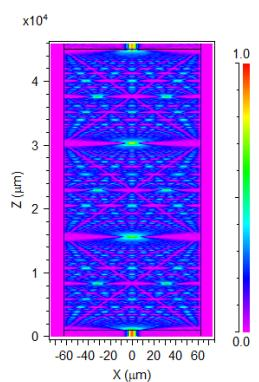
\includegraphics[keepaspectratio,alt={image}]{images/26d4d031cf8080be4fa7f4197ba01f695aa837ae6dca3cc1ab90ee8bfeede0af.jpg}}

\pandocbounded{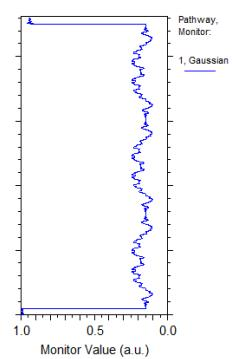
\includegraphics[keepaspectratio,alt={image}]{images/1d7d70aca30263bf893b58264fd018d35143fa3fc942849a87e463537e649809.jpg}}

\begin{enumerate}
\def\labelenumi{(\alph{enumi})}
\tightlist
\item
\end{enumerate}

\pandocbounded{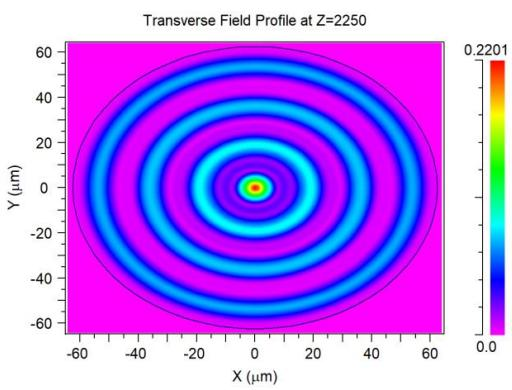
\includegraphics[keepaspectratio,alt={image}]{images/0b137e4ae1f7a6dc3315a633a8086b74d614fac091bcec511f4ef13ba883eae8.jpg}}

\begin{enumerate}
\def\labelenumi{(\alph{enumi})}
\setcounter{enumi}{1}
\tightlist
\item
\end{enumerate}

\pandocbounded{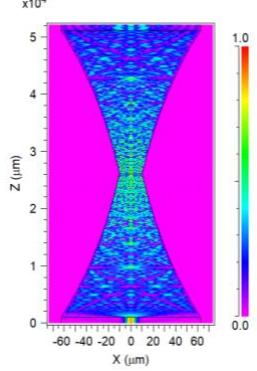
\includegraphics[keepaspectratio,alt={image}]{images/eae8e4eab1770d41e35fc46aadb7f85792d388964aa3a33e845b54cc70af7321.jpg}}

\pandocbounded{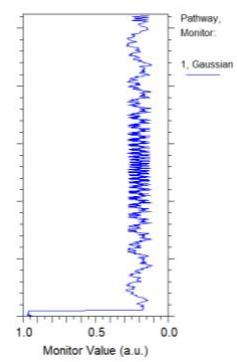
\includegraphics[keepaspectratio,alt={image}]{images/bd1f0f474058bed4a4ae9bcd4a59f0516e200d13316a5f002012e7b766b72174.jpg}}

\begin{enumerate}
\def\labelenumi{(\alph{enumi})}
\setcounter{enumi}{2}
\tightlist
\item
\end{enumerate}

\pandocbounded{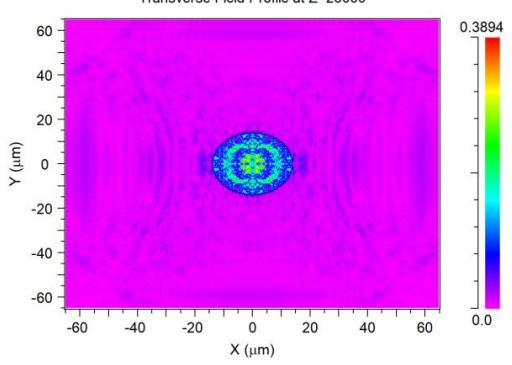
\includegraphics[keepaspectratio,alt={image}]{images/ee0bc2e2e905639fa476062f6ab630eb9d8d98281604fc9ed8d862cb33badefb.jpg}}

\begin{enumerate}
\def\labelenumi{(\alph{enumi})}
\setcounter{enumi}{3}
\tightlist
\item
\end{enumerate}

Transverse Field Profile at Z=25000

\pandocbounded{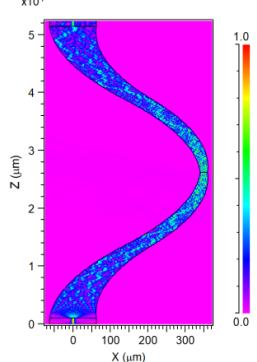
\includegraphics[keepaspectratio,alt={image}]{images/8d73d21bbe46aef78f0772da8836d97645f30ee997447523ae9859efb40b3cba.jpg}}

\pandocbounded{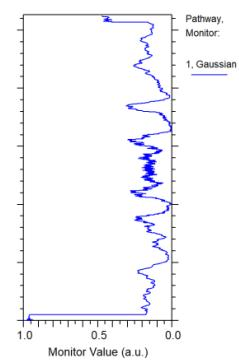
\includegraphics[keepaspectratio,alt={image}]{images/1890adfea1af659ab2337e89f787528339ad39eb5080a3bf87df0df322c8a18b.jpg}}

\begin{enumerate}
\def\labelenumi{(\alph{enumi})}
\setcounter{enumi}{4}
\tightlist
\item
\end{enumerate}

\pandocbounded{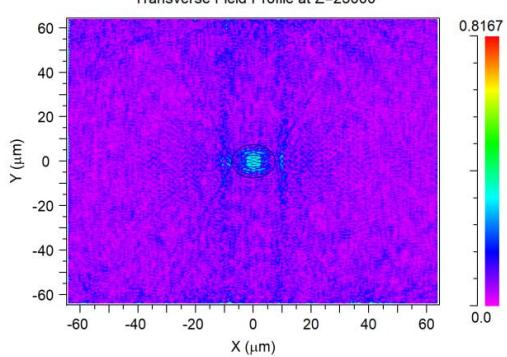
\includegraphics[keepaspectratio,alt={image}]{images/360a5f2bf233f2bd059aaa1aeba91cc03c0768017b0975d233a852d258f27a9d.jpg}}

\begin{enumerate}
\def\labelenumi{(\alph{enumi})}
\setcounter{enumi}{5}
\tightlist
\item
\end{enumerate}

图3 三种结构的纵向光场分布 (a) 无芯光纤 (c) 锥形无芯光纤 (e)
U型锥形无芯光纤三种结构的横向光场分布 (b) 无芯光纤 (d) 锥形无芯光纤 (f)
U型锥形无芯光纤

\subsection{1.3
传感系统设计原理}\label{ux4f20ux611fux7cfbux7edfux8bbeux8ba1ux539fux7406}

为了直观显示待测透明液体的浓度值，设计了光纤传感系统。系统包括：光纤传感模块（光源和
SNS
传感探头）、单片机控制模块、实现各种功能的硬件电路（光电检测模块、信号放大与A/D转换电路）以及显示模块，整个系统设计的原理框图如图4所示。光纤传感模块产生的光信号传递到光电检测模块，将光信号转换成电信号后传送到下一级的放大与A/D转换电路，处理后的信号通过通信接口连接到控制模块，由控制模块计算并最后在显示模块上实时显示出透明液体的浓度值。

\pandocbounded{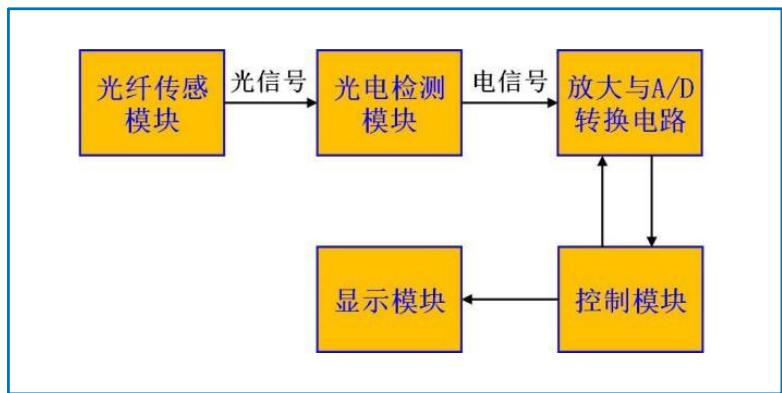
\includegraphics[keepaspectratio,alt={image}]{images/b75ec4c9769d37f57a3f49f84ecc0fa1f1a44f71b8b8df199068d0cee8b1dbac.jpg}}

图 4 传感系统示意图

在本传感系统中，控制模块采用 STM32F103 系列单片机，是基于 ARM
Cortex-M3内核开发的32位闪存的单片微型计算机（微控制器）；选用 ALIENTEK
MiniSTM32开发板；采用 TFT-LCD 液晶显示。本设计中 STM32 的软件开发环境为
Keil MDK，Keil是一款可以支持 Cortex-M3
内核标准的仿真编译软件，可以使用C语言进行编译，J-LINK在线调试，操作简单方便。调试完成后将程序烧入
STM32芯片。

\subsection{2.
实验方案、步骤及其结果分析}\label{ux5b9eux9a8cux65b9ux6848ux6b65ux9aa4ux53caux5176ux7ed3ux679cux5206ux6790}

⚫ 实验器材：单模光纤(SMF-28)，无芯光纤
(CL1010-A)，剥线钳，切割刀，酒精，无纺 布 ， 熔 接 机 （INNO IFS-15M）
， 宽 带 光 源 （NKT DK-3460） ， 光 谱 仪（Yokogawa AQ6370C），1550nm
激光器（KF-184A），功率计（JW3208），3dB耦合器，熔融拉锥机（AFBT-6000），扫描电镜(SEM:
Quanta FEG250)，不同浓度的盐水

\subsection{2.1 基于
NCF的光纤传感探头制作及其特性研究}\label{ux57faux4e8e-ncfux7684ux5149ux7ea4ux4f20ux611fux63a2ux5934ux5236ux4f5cux53caux5176ux7279ux6027ux7814ux7a76}

⚫ 实验方案及其步骤：

本实验选用直径为
125μm的CL1010-A无芯光纤作为传感探头的主要元件，切割长度为 4.4cm。

\subsection{（1）处理光纤端面}\label{ux5904ux7406ux5149ux7ea4ux7aefux9762}

取一根
2米长的单模光纤跳线，用剪刀截成两段，带连接头的两端留作测试备用，剪开的部分需要跟无芯光纤进行熔接。用剪刀将保护套剥开，再用剥线钳剥离光纤护套，控制剥线长度在4cm左右，使用无纺布蘸取少量酒精，顺光纤轴向擦去光纤表面残留的碎屑，再使用光纤切割刀将光纤端面切平整。无芯光纤的端面处理与上面步骤相同。

\subsection{（2）熔接单模光纤与无芯光纤}\label{ux7194ux63a5ux5355ux6a21ux5149ux7ea4ux4e0eux65e0ux82afux5149ux7ea4}

将处理好端面的无芯光纤与单模光纤放入熔接机的 V
型槽，合上压板，关闭防风盖。按下SET键，此时熔接机的显示屏会显示光纤端面的平整情况以及两光纤放置的位置情况，如果符合要求，再次按下SET键，电极进行电弧放电，熔接完毕。同理，继续熔接无芯光纤与另外一根单模光纤，形成
SNS光纤结构的传感探头。

\subsection{（3）点胶封装}\label{ux70b9ux80f6ux5c01ux88c5}

使用熔融拉锥机的封装功能进行封装。打开拉锥机电源开关，在电脑桌面上打开程序
进入拉锥机的工作界面。将制作好的
光纤传感探头放置在夹具上，取一个石英半管放在封装架上，点击``封装''键，封装架自动移动到SNS传感探头的下方。用牙签取少量紫外线凝固胶（UV胶），分别适量滴在石英半管两端，期间注意尽量保持半管不动，最后用紫外灯照射直到胶水凝固，光纤传感探头部分完成封装。

\subsection{（4）测试传感探头的传感特性}\label{ux6d4bux8bd5ux4f20ux611fux63a2ux5934ux7684ux4f20ux611fux7279ux6027}

将传感探头放置在玻璃皿中固定好，一端连接宽带光源，另一端连接光谱仪。光从宽带光源(波长范围
1525-1610nm)耦合进传感探头。透射光谱由分辨率为 0.02nm的光谱仪(Yokogawa
AQ6370C)记录。通过光谱仪测量不同浓度下锥形无芯光纤透射谱变化规律，如图
5（a）和（b）所示。为了直观显示透明液体的浓度值，将光源波长固定在1550nm处，测量功率变化与浓度的关系，如图
5（c）和（d）中所示。光从
1550nm激光器发出，进入3dB耦合器，耦合器一端连接功率计1用来监测光源的波动，另一端连接传感探头，透明液体的浓度发生变化时，传感探头输出的光功率用功率计
2来测量。

以1\%为步长，配置好0～15\%的盐水溶液，依次倒入玻璃器皿，对探头的传感特性进行测试。当测完一种浓度的溶液后，用针管将测完的溶液吸走，再用新的针管吸取酒精慢慢清洗传感区域多次，这样可以把残留的溶液彻底清除干净，防止对下一种浓度溶液的测量产生影响。

\pandocbounded{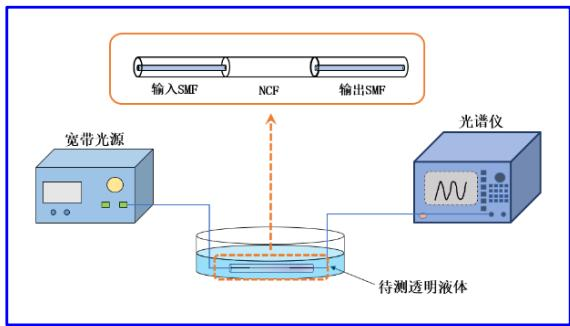
\includegraphics[keepaspectratio,alt={image}]{images/bca886bdd40fd6a3cf55243ec5e97c74eb491cda0c758ab0ea7f10be8f780dae.jpg}}

（a）

\pandocbounded{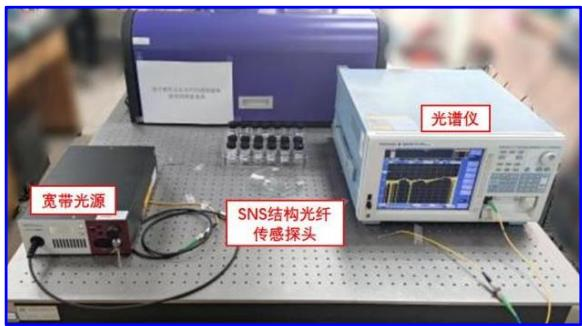
\includegraphics[keepaspectratio,alt={image}]{images/eb1333f29007ece37012d5406dc47e851d9c7a0c1c3d65f0891dc057c61a4bc2.jpg}}

（b）

\pandocbounded{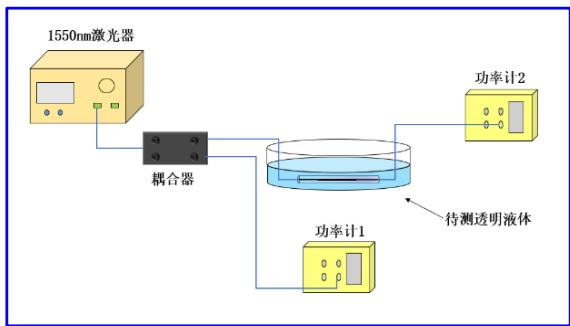
\includegraphics[keepaspectratio,alt={image}]{images/c093f750bb2effff4fc203b37b99629ecafa83bd16a46d65948b8721eda39ef5.jpg}}

（c）

\pandocbounded{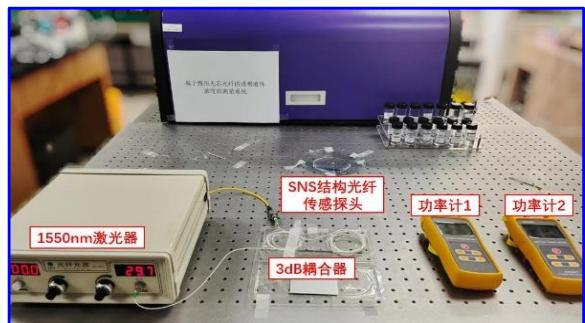
\includegraphics[keepaspectratio,alt={image}]{images/d74bd8272859c7b84d05bd6977043d691efe4e7d4fed66f0a4a6268524944e64.jpg}}

（d）

图5 基于NCF传感探头的传感特性测试

（a）测量透射光谱装置示意图（b）测量透射光谱装置实物图

（c）透射功率装置示意图（d）透射功率装置实物图

\subsection{⚫
传感结果及其分析：}\label{ux4f20ux611fux7ed3ux679cux53caux5176ux5206ux6790}

图6为基于NCF的传感探头在不同浓度的透明盐水溶液中的透射光谱。

\pandocbounded{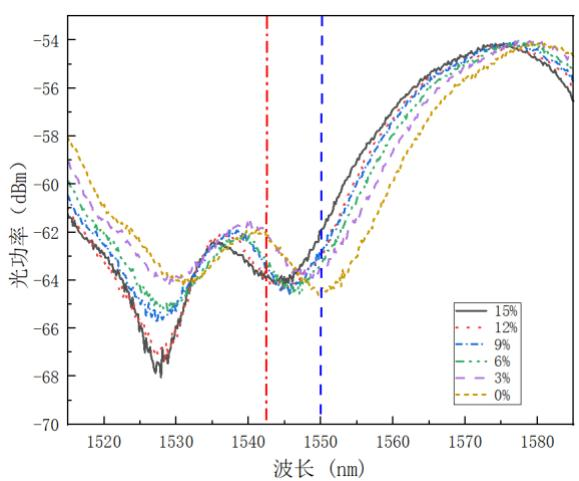
\includegraphics[keepaspectratio,alt={image}]{images/ef3ebad384eaddad49ec3c88e8b31a735f406f43c8944f40c22eaa3992790aac.jpg}}

图6 基于NCF的传感探头在不同浓度的透明盐水溶液中的透射光谱

从图中可以看到，在 1550nm
处（图中竖条蓝线位置），随着盐水溶液浓度的增加，传感器输出端的光功率不断增大。如果波长选在
1542.5nm
处（图中竖条红线位置），则随着透明盐水溶液浓度的增加，输出光功率不断减小。本实验中测量输出功率随着透明液体的浓度变化时，选择
1550nm的光源。

基于NCF的光纤传感探头在盐水溶液中的功率随浓度变化的数据如表 2所示。

表2 SNS结构光纤传感探头在不同浓度的盐水溶液中的功率

{\def\LTcaptype{none} % do not increment counter
\begin{longtable}[]{@{}|l|l|l|@{}}
\toprule\noalign{}
\endhead
\bottomrule\noalign{}
\endlastfoot
\hline
浓度(盐)(\%) & 光源功率(uW) & 传感探头功率(uW) \\
\hline
1 & 193.6 & 4.857 \\
\hline
2 & 193.8 & 4.930 \\
\hline
3 & 193.6 & 4.942 \\
\hline
4 & 193.6 & 4.995 \\
\hline
5 & 193.7 & 5.025 \\
\hline
6 & 193.7 & 5.079 \\
\hline
7 & 193.6 & 5.100 \\
\hline
8 & 193.8 & 5.133 \\
\hline
9 & 193.6 & 5.202 \\
\hline
10 & 193.5 & 5.252 \\
\hline
11 & 193.6 & 5.293 \\
\hline
12 & 193.7 & 5.321 \\
\hline
13 & 193.8 & 5.393 \\
\hline
14 & 193.6 & 5.403 \\
\hline
15 & 193.5 & 5.422 \\
\hline
\end{longtable}
}

使用 Origin 软件对所得实验数据拟合，绘制出基于 NCF
的光纤传感探头功率随浓度变化曲线如图7所示。

\pandocbounded{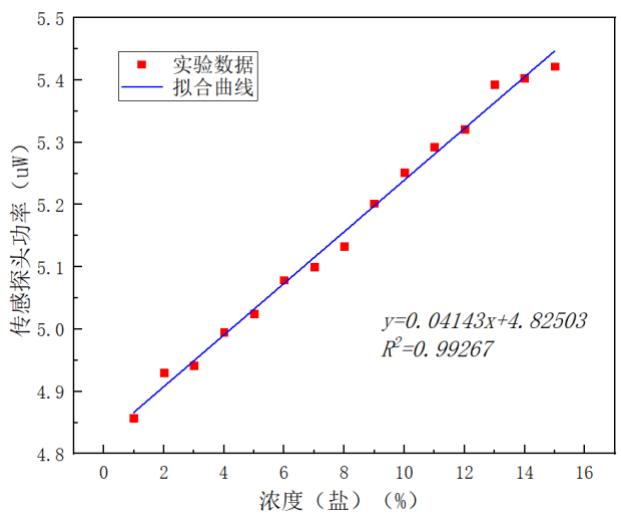
\includegraphics[keepaspectratio,alt={image}]{images/d19803dc734d1875b5e87046000444ab478ca69573af47b2f4d4028356069b00.jpg}}

图7 基于 NCF的光纤传感探头在盐水溶液中功率随浓度变化的曲线

可以看到，在盐水溶液中，基于 NCF
的光纤传感探头功率随浓度变化呈现出良好的线性关系。其拟合的线性关系为
y=0.04143x+4.82503，灵敏度为 41.43nW/\%，相关系数为 0.9927。

\subsection{2.2 基于锥形
NCF的传感探头制作及其特性研究}\label{ux57faux4e8eux9525ux5f62-ncfux7684ux4f20ux611fux63a2ux5934ux5236ux4f5cux53caux5176ux7279ux6027ux7814ux7a76}

\subsection{⚫
实验方案及其步骤：}\label{ux5b9eux9a8cux65b9ux6848ux53caux5176ux6b65ux9aa4}

\subsection{（1）制作锥形NCF的传感探头}\label{ux5236ux4f5cux9525ux5f62ncfux7684ux4f20ux611fux63a2ux5934}

为增加传感探头的灵敏度，本实验对NCF进行拉锥处理。用熔融拉锥机制作锥形NCF。参数设置如表3所示。待拉伸长度达到3500μm时，点击停止。随后对光纤传感探头部分进行封装。

表3 拉锥机主要参数设置

{\def\LTcaptype{none} % do not increment counter
\begin{longtable}[]{@{}|l|l|@{}}
\toprule\noalign{}
\endhead
\bottomrule\noalign{}
\endlastfoot
\hline
\multicolumn{2}{@{}l@{}}{%
拉伸台设置} \\
\hline
拉伸速度 V1 (um/sec) & 160 \\
\hline
拉伸速度 V2 (um/sec) & 160 \\
\hline
点动速度 (um/sec) & 300 \\
\hline
马达加速度 (um/sec\^{}\{2\}) & 11000 \\
\hline
马达减速度 (um/sec\^{}\{2\}) & 11000 \\
\hline
初始距离 (um) & 7000 \\
\hline
\multicolumn{2}{@{}l@{}}{%
监控参数设置} \\
\hline
CR (0-99.9\%) & 42 \\
\hline
耦合周期 (0-400) & 0 \\
\hline
H\_\{2\}流量 (SCCM) & 160 \\
\hline
\multicolumn{2}{@{}l@{}}{%
附加设置} \\
\hline
预拉速度 V (um/sec) & 200 \\
\hline
预拉距离 (um) & 520 \\
\hline
\end{longtable}
}

\subsection{（2）测试基于锥形NCF传感探头的特性}\label{ux6d4bux8bd5ux57faux4e8eux9525ux5f62ncfux4f20ux611fux63a2ux5934ux7684ux7279ux6027}

图8（a）为实验装置示意图，图
8（b）为实验装置实物图。除了光纤探头采用锥形NCF之外，其他实验装置与图
5（c）和（d）相同。实验中待测液体还是 0～15\%的盐水溶液，浓度步长为
1\%。

\pandocbounded{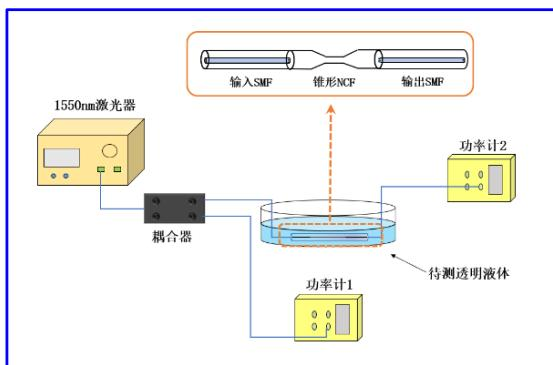
\includegraphics[keepaspectratio,alt={image}]{images/9298a261eed58ffc97cf87607de5cb0a9e40e9131d2ac1663a677b01b8c7757d.jpg}}

（a）

\pandocbounded{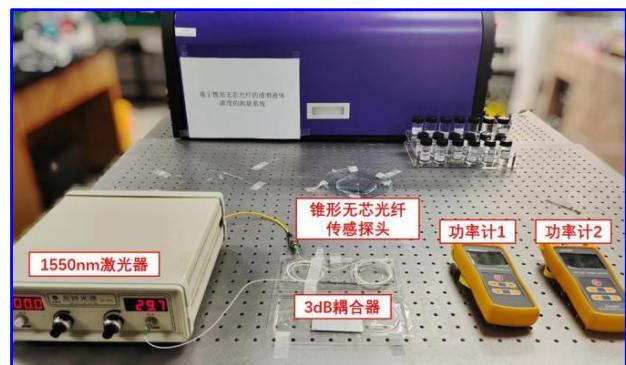
\includegraphics[keepaspectratio,alt={image}]{images/6d97dc7bc84055f700af5b3bf49837a51b08abfe9dbbca19070a70d6e7503ba7.jpg}}

（b）

图 8 基于锥形NCF传感探头的特性测试 （a）实验装置示意图
（b）实验装置实物图

\subsection{⚫
传感结果及其分析：}\label{ux4f20ux611fux7ed3ux679cux53caux5176ux5206ux6790-1}

基于锥形NCF的传感探头在不同浓度的盐水溶液中的功率随浓度变化的数据如表4所示。

表4 基于锥形NCF的传感探头在不同浓度的盐水溶液中的功率

{\def\LTcaptype{none} % do not increment counter
\begin{longtable}[]{@{}|l|l|l|@{}}
\toprule\noalign{}
\endhead
\bottomrule\noalign{}
\endlastfoot
\hline
浓度(盐)(\%) & 光源功率(uW) & 传感探头功率(uW) \\
\hline
1 & 193.7 & 2.397 \\
\hline
2 & 193.6 & 2.424 \\
\hline
3 & 193.7 & 2.451 \\
\hline
4 & 193.8 & 2.544 \\
\hline
5 & 193.5 & 2.573 \\
\hline
6 & 193.6 & 2.649 \\
\hline
7 & 193.6 & 2.712 \\
\hline
8 & 193.8 & 2.779 \\
\hline
9 & 193.6 & 2.847 \\
\hline
10 & 193.7 & 2.888 \\
\hline
11 & 193.7 & 2.938 \\
\hline
12 & 193.6 & 2.972 \\
\hline
13 & 193.8 & 3.061 \\
\hline
14 & 193.6 & 3.136 \\
\hline
15 & 193.6 & 3.184 \\
\hline
\end{longtable}
}

使用 Origin 软件对所得实验数据进行拟合，所得基于锥形 NCF
的光纤传感探头功率随浓度变化曲线如图 9所示。

\pandocbounded{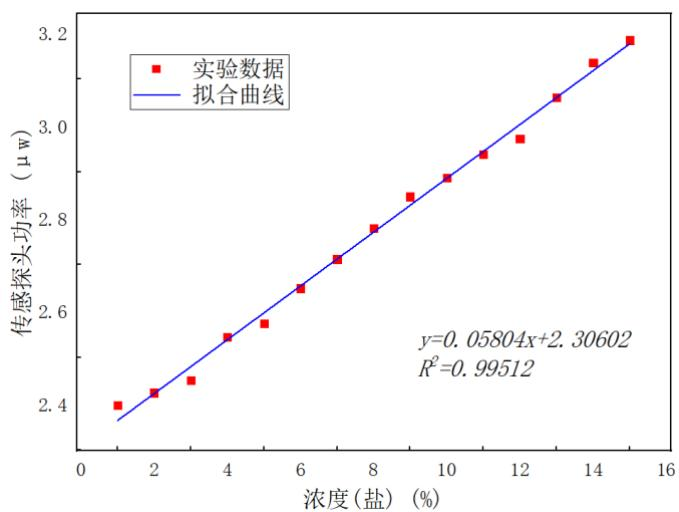
\includegraphics[keepaspectratio,alt={image}]{images/5d4db33bbedac6fcc777b30f7c4cb39b9c85e928c372fb6c1f434f03202b837e.jpg}}

图9 基于锥形NCF的传感探头在盐水溶液中功率随浓度变化的曲线

由此可知，在盐水溶液中，基于锥形NCF的传感探头功率随浓度变化的拟合线性关系为
y=0.05804x+2.30602，其灵敏度为 58.04nW/\%，相关系数为
0.9951。将该实验结果与基于NCF的传感结构的实验结果比较可知，传感器的灵敏度提高到基于NCF传感结构的1.4倍。

\subsection{2.3 基于 U型锥形
NCF传感探头的制作及其性能研究}\label{ux57faux4e8e-uux578bux9525ux5f62-ncfux4f20ux611fux63a2ux5934ux7684ux5236ux4f5cux53caux5176ux6027ux80fdux7814ux7a76}

\subsection{⚫
实验方案及其步骤：}\label{ux5b9eux9a8cux65b9ux6848ux53caux5176ux6b65ux9aa4-1}

（1）将未封装的锥形 NCF 传感探头的锥形部分弯曲大约 60°，制作成 U
型锥形NCF传感探头，并且固定在玻璃皿中。为了对比NCF、锥形NCF以及U型锥型NCF形貌上的差别，使用扫描电镜
SEM对上述三种结构的光纤进行了观测，其结果如图
10所示，从图(a)和图(b)中可以看到，NCF的直径约为 125μm，锥形
NCF的直径明显变细，约为20μm，图（c）为 U型锥形NCF的形状。

\subsection{（2）测试U型锥形NCF传感探头的传感特性}\label{ux6d4bux8bd5uux578bux9525ux5f62ncfux4f20ux611fux63a2ux5934ux7684ux4f20ux611fux7279ux6027}

测试 U 型锥形 NCF
传感探头的传感特性的实验装置如图（11）所示。除了光纤探头采用 U型锥形
NCF之外，其他实验装置与图 5（c）和（d）相同。以
1\%为步长，配制好0～15\%的盐水溶液。

\pandocbounded{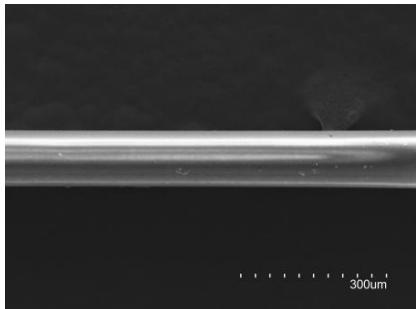
\includegraphics[keepaspectratio,alt={image}]{images/25d42e5494aa7dfa8b60f3577112169a0423732387515c3f10cd4472533fe336.jpg}}

（a）

\pandocbounded{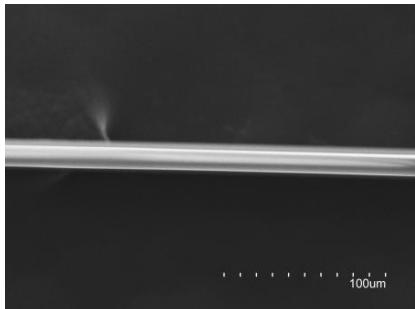
\includegraphics[keepaspectratio,alt={image}]{images/87009f8d978d170d190dc43681ac6283d41588b0ce98fbbbfee235366e371869.jpg}}

（b）

\pandocbounded{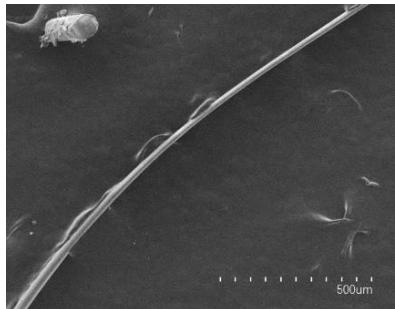
\includegraphics[keepaspectratio,alt={image}]{images/68003876b6827df6fbebabb55be2320aefb3a815cfd2bd256d4ed847ef769e6e.jpg}}

（c）

图 10 三种结构的 NCF 的 SEM 照片 （a）NCF（b）锥形 NCF（c）U 型锥形 NCF

\pandocbounded{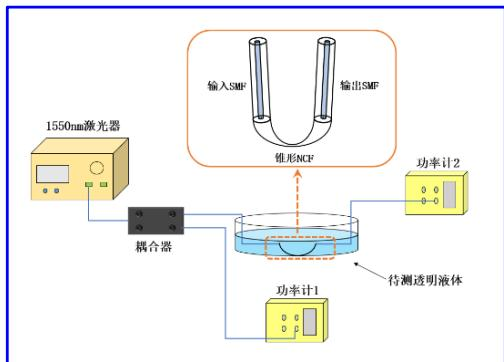
\includegraphics[keepaspectratio,alt={image}]{images/b7c1d50206dbb95ffde559b0cb677ef888ea393d2a8be66b4460e35efa243163.jpg}}

（a）

\pandocbounded{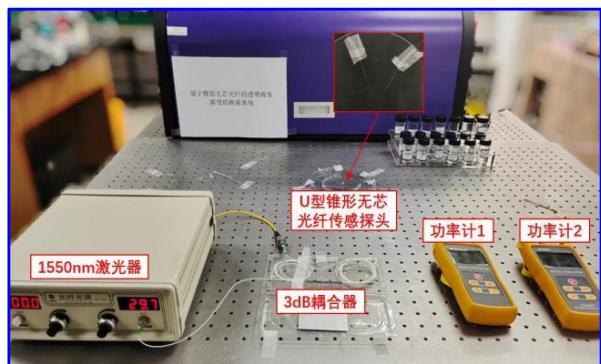
\includegraphics[keepaspectratio,alt={image}]{images/7a1ae1ca112e5d81f4c7de22ffd980ad536ea2e93591c47626d468458a84d713.jpg}}

（b）

图11 基于U型锥形NCF的传感探头的特性测试 （a）实验装置示意图
（b）实验装置实物图

\subsection{⚫
传感结果及其分析：}\label{ux4f20ux611fux7ed3ux679cux53caux5176ux5206ux6790-2}

U型锥形NCF传感探头在不同浓度的盐水溶液中的功率随浓度变化的数据如表5所示。

表5 U型锥形无芯光纤传感探头在不同浓度的盐水溶液中的功率

{\def\LTcaptype{none} % do not increment counter
\begin{longtable}[]{@{}|l|l|l|@{}}
\toprule\noalign{}
\endhead
\bottomrule\noalign{}
\endlastfoot
\hline
浓度(盐)(\%) & 光源功率(uW) & 传感探头功率(uW) \\
\hline
1 & 193.6 & 2.491 \\
\hline
2 & 193.5 & 2.389 \\
\hline
3 & 193.7 & 2.248 \\
\hline
4 & 193.8 & 2.103 \\
\hline
5 & 193.7 & 2.059 \\
\hline
6 & 193.6 & 2.017 \\
\hline
7 & 193.6 & 1.831 \\
\hline
8 & 193.5 & 1.682 \\
\hline
9 & 193.6 & 1.538 \\
\hline
10 & 193.5 & 1.447 \\
\hline
11 & 193.6 & 1.359 \\
\hline
12 & 193.7 & 1.206 \\
\hline
13 & 193.5 & 1.13 \\
\hline
14 & 193.6 & 0.9836 \\
\hline
15 & 193.7 & 0.9059 \\
\hline
\end{longtable}
}

使用 Origin 软件对所得实验数据进行拟合，所得 U 型锥形 NCF
传感探头功率随浓度变化曲线如图12所示。

\pandocbounded{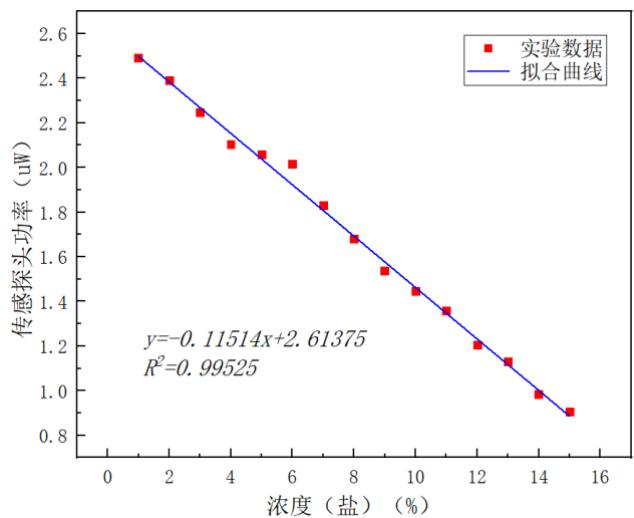
\includegraphics[keepaspectratio,alt={image}]{images/6b99d8a93569b872319ae8186c60d5567d85c49be1de477f79925b3f0f2638b0.jpg}}

图12 U型锥形无芯光纤传感探头在盐水溶液中功率随浓度的变化

由此可知，在盐水溶液中，U型锥形NCF传感探头功率随浓度变化的拟合线性关系为
y=-0.11514x+2.61375，其灵敏度为 115.14nW/\%，相关系数为
0.9953。将该实验结果与基于NCF的传感探头的传感效果相比，传感器的灵敏度又提高了
1倍左右。所以采用U型锥形NCF传感探头，可以使得液体传感器的灵敏度大幅提高，该实验结果与理论分析的结果基本一致。

\subsection{⚫ 误差分析：}\label{ux8befux5deeux5206ux6790}

该实验的误差是指实际液体浓度值与从功率计所测光功率随液体浓度变化的拟合线性关系中得到的液体浓度值之间的差别。造成误差的原因是光源的不稳定性，以及置换不同浓度的液体时液体对光纤探头的冲击力也会对输出光功率造成影响。所以实验中采用3dB耦合器监测光源的功率变化，如果变化太大，就通过调节光源的电流让其稳定在初始值。置换不同浓度的溶液时，尽可能缓慢，保持光纤探头的初始状态不变。通过对所测的全部数据进行分析发现，测量盐水溶液时：平均误差为±0.218\%，最大误差为0.824\%，最小误差为
0.048\%。从误差分析中可以看到，U 型锥形 NCF
传感探头的测量误差很小，完全可以满足实际应用的需求。

\subsection{2.4 基于 U型锥形
NCF的液体浓度传感系统}\label{ux57faux4e8e-uux578bux9525ux5f62-ncfux7684ux6db2ux4f53ux6d53ux5ea6ux4f20ux611fux7cfbux7edf}

⚫
实验器材：1550nm激光器（KF-184A），3dB耦合器，功率计（JW3208），U型锥形NCF传感探头，STM32F103系列开发板，1GHz光电探测器，AD620电路模块，ADS115电路模块，不同浓度的盐水和酒精

\subsection{⚫
实验方案及其步骤：}\label{ux5b9eux9a8cux65b9ux6848ux53caux5176ux6b65ux9aa4-2}

为能直观显示所测透明液体的浓度值，本实验在
U型锥形NCF传感装置的设计基础上加入解调装置，包括单片机控制模块、光电检测模块、信号放大与
A/D转换电路以及显示模块，如图13（a）所示，数据处理显示模块的程序流程如图
13（b）所示。型锥形
传感探头输出的光信号由光检测模块接收后，将光信号转化为电信号，传送到下一级的放大与
A/D转换电路，处理后的信号通过通信接口连接到控制模块，由控制模块计算并最后在显示模块上实时显示浓度值，实现透明液体的浓度测量。实验装置示意图和实物图如图
14（a）和（b）所示。

实验中首先打开1550nm激光器，用
3dB耦合器一端连接功率计监测光源的稳定性。3dB耦合器的另外一端连接光电探测器，U型锥形NCF传感探头固定在玻璃皿中，将配置好的不同浓度的透明液体加入玻璃皿，观察单片机显示模块示数，待示数稳定后进行记录。

\pandocbounded{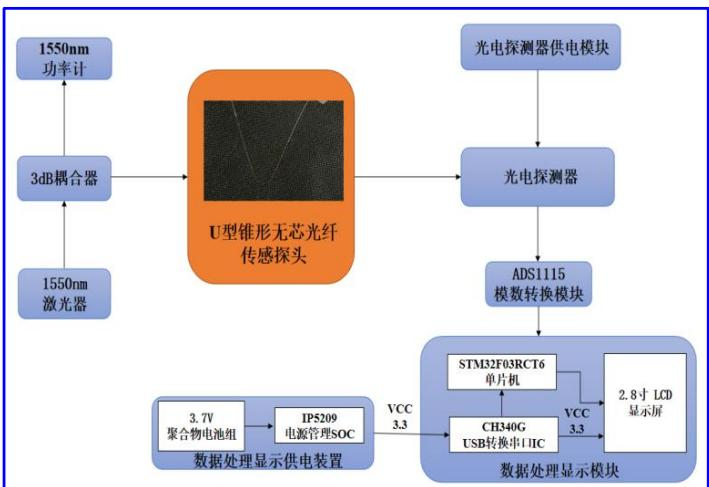
\includegraphics[keepaspectratio,alt={image}]{images/5504389f40045a9172a50d6b2d955fba2a90cdcac91189964698265e76a59316.jpg}}

（a）

\pandocbounded{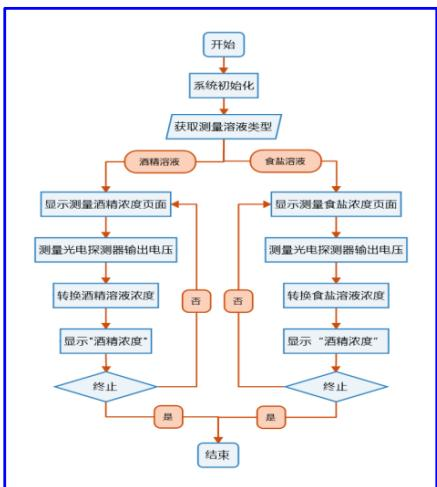
\includegraphics[keepaspectratio,alt={image}]{images/e1baa9bfca84021ac0c660be098869df46a5eed8b9cf030708a3fa1de17d5d22.jpg}}

（b）

图13 透明液体浓度测量系统（a）总体系统流程

（b）数据处理显示模块流程

\pandocbounded{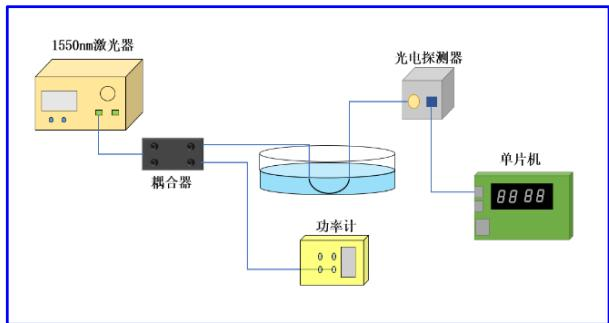
\includegraphics[keepaspectratio,alt={image}]{images/4e7f76d3388b41ca941df55b46194859c2ac7e33fd2fdf98fe1c6836b4c67616.jpg}}

（a）

\pandocbounded{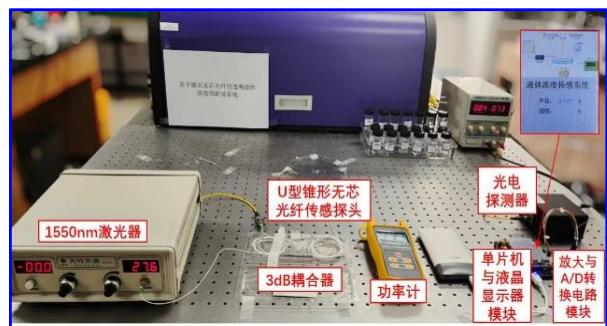
\includegraphics[keepaspectratio,alt={image}]{images/53186739fed1211a8f7afaa21e3ba4cdf41d6ddab97c5b2448683683e5e7ac1f.jpg}}

（b）

图 14 基于 U型锥形NCF传感探头的液体浓度测量系统

（a）实验装置示意图 （b）实验装置实物图

\subsection{⚫
实验结果及其分析：}\label{ux5b9eux9a8cux7ed3ux679cux53caux5176ux5206ux6790}

实时测量透明液体浓度，实际液体浓度值和单片机所显示的测量浓度值及两者间的误差如表6所示。

表6 液体浓度实际值、测量值和误差

{\def\LTcaptype{none} % do not increment counter
\begin{longtable}[]{@{}|l|l|l|l|l|l|@{}}
\toprule\noalign{}
\endhead
\bottomrule\noalign{}
\endlastfoot
\hline
\multicolumn{3}{@{}l}{%
盐水溶液} & \multicolumn{3}{l@{}}{%
酒精溶液} \\
\hline
实际浓度值 & 测量浓度值 & 误差 & 实际浓度值 & 测量浓度值 & 误差 \\
\hline
0.00\% & 0.01\% & 0.01\% & 5.00\% & 4.99\% & -0.01\% \\
\hline
1.00\% & 0.98\% & -0.02\% & 10.00\% & 9.98\% & -0.02\% \\
\hline
2.00\% & 2.01\% & 0.01\% & 15.00\% & 14.98\% & -0.02\% \\
\hline
3.00\% & 3.03\% & 0.03\% & 20.00\% & 19.97\% & -0.03\% \\
\hline
4.00\% & 3.94\% & -0.06\% & 25.00\% & 24.98\% & -0.02\% \\
\hline
5.00\% & 5.04\% & 0.04\% & 30.00\% & 29.96\% & -0.04\% \\
\hline
6.00\% & 6.05\% & 0.05\% & 35.00\% & 34.95\% & -0.05\% \\
\hline
7.00\% & 7.07\% & 0.07\% & 40.00\% & 39.94\% & -0.06\% \\
\hline
8.00\% & 7.95\% & -0.05\% & 45.00\% & 44.92\% & -0.08\% \\
\hline
9.00\% & 9.08\% & 0.08\% & 50.00\% & 49.93\% & -0.07\% \\
\hline
10.00\% & 10.09\% & 0.09\% & 55.00\% & 54.91\% & -0.09\% \\
\hline
11.00\% & 10.90\% & -0.10\% & 60.00\% & 59.89\% & -0.11\% \\
\hline
12.00\% & 12.05\% & 0.05\% & 65.00\% & 64.92\% & -0.08\% \\
\hline
13.00\% & 13.12\% & 0.12\% & 70.00\% & 69.91\% & -0.09\% \\
\hline
14.00\% & 14.17\% & 0.17\% & 75.00\% & 74.90\% & -0.10\% \\
\hline
15.00\% & 15.23\% & 0.23\% & 80.00\% & 79.88\% & -0.12\% \\
\hline
& & & 85.00\% & 84.85\% & -0.15\% \\
\hline
& & & 90.00\% & 89.86\% & -0.14\% \\
\hline
& & & 95.00\% & 94.82\% & -0.18\% \\
\hline
\end{longtable}
}

\subsection{⚫ 误差分析：}\label{ux8befux5deeux5206ux6790-1}

该实验中，误差是指系统显示液体浓度值与实际液体浓度值之间的偏差。误差来源于光源的不稳定性和置换不同浓度的液体时，对光纤探头的冲击力。实验中尽管采取方法减小这些误差，但是不能消除。取多组不同液体浓度的数据，对比分析系统显示液体浓度值与液体浓度标准值之间的差异，当盐水溶液在
0～15\%的浓度范围内：平均误差为 0.07\%，最大误差为 0.23\%，最小误差为
0.01\%。当酒精溶液在 5\%～95\%的浓度范围内：平均误差为
0.08\%，最大误差为 0.18\%，最小误差为 0.01\%。此种基于锥形
NCF的透明液体浓度传感器与一定范围的实际液体浓度的平均误差范围很小，具有很好的准确性和实时性。

\subsection{3.项目创新与特色}\label{ux9879ux76eeux521bux65b0ux4e0eux7279ux8272}

\subsection{3.1
SNS结构光纤传感探头的优势}\label{snsux7ed3ux6784ux5149ux7ea4ux4f20ux611fux63a2ux5934ux7684ux4f18ux52bf}

相较于传统的浓度传感器，光纤传感器价格低廉，体积小、重量轻且制备简单。

\subsection{3.2 U型锥形
NCF传感探头提高传感精度}\label{uux578bux9525ux5f62-ncfux4f20ux611fux63a2ux5934ux63d0ux9ad8ux4f20ux611fux7cbeux5ea6}

一般情况下，基于 NCF
的传感探头灵敏度不够高（本实验中测量盐水溶液的浓度灵敏度为：41.43nW/\%），而采用的基于锥形NCF的传感探头能够很好的提高传感器的灵敏度（腰锥直径为20μm，灵敏度为58.04nW/\%），基于U型锥形NCF的传感探头具有最高的灵敏度（115.14nW/\%）。

\subsection{3.3
系统可以实现液体浓度实时显示}\label{ux7cfbux7edfux53efux4ee5ux5b9eux73b0ux6db2ux4f53ux6d53ux5ea6ux5b9eux65f6ux663eux793a}

本实验系统中通过光电探测器将接收到的光信号转换为电信号，由电路模块放大并转换为数字信号，通过对单片机进行编程，使其经计算后在外接屏幕上实时显示被测液体浓度的数值。系统简单、小巧，易于控制且适用范围广。为该基于
U 型锥形 NCF 的透明液体浓度传感器的实际应用推广奠定了基础。

\subsection{4.结论}\label{ux7ed3ux8bba}

本实验基于 型锥形
的传感特性研制了一种测量透明液体浓度的传感系统，可直接将待测液体置入装有光纤传感探头的玻璃皿，通过单片机以及液晶显示模块实时显示待测透明液体的浓度值，盐水的测量范围为
0 到 15\%，酒精的测量范围为 0
到95\%，测量范围较为广泛，且可以扩展实现更多种类的透明液体浓度的测量。通过对NCF拉锥弯曲处理，能显著提高测试灵敏度，对于盐水溶液的灵敏度可以从41.43nW/\%增加到115.14nW/\%。这种基于U型锥形NCF的透明液体浓度传感器简单小巧且适用范围广，提高了液体浓度测量的灵敏度与稳定性。

\subsection{5.制作成本（明细）}\label{ux5236ux4f5cux6210ux672cux660eux7ec6}

{\def\LTcaptype{none} % do not increment counter
\begin{longtable}[]{@{}|l|l|l|l|@{}}
\toprule\noalign{}
\endhead
\bottomrule\noalign{}
\endlastfoot
\hline
名称 & 数量 & 单价(元) & 总价(元) \\
\hline
一次性注射器 & 20 & 1.64 & 32.8 \\
\hline
3米SMF & 3 & 30 & 90 \\
\hline
1米NCF & 1 & 150 & 150 \\
\hline
酒精灯 & 1 & 24 & 24 \\
\hline
3dB耦合器 & 1 & 100 & 100 \\
\hline
石英半管 & 20 & 1.5 & 30 \\
\hline
UV胶 & 1 & 37.88 & 37.88 \\
\hline
模数转换模块 & 1 & 30 & 30 \\
\hline
STM32单片机、显示屏 & 1 & 318 & 318 \\
\hline
总计 & \multicolumn{3}{l@{}}{%
812.68元} \\
\hline
\end{longtable}
}

\end{document}
